\documentclass[epsfig,10pt,fullpage]{article}

\newcommand{\LabNum}{6}
\newcommand{\CommonDocsPath}{../../common/docs}
\input{\CommonDocsPath/preamble.tex}

\begin{document}

\centerline{\huge Embedded Systems}
~\\
\centerline{\huge Laboratory Exercise \LabNum}
~\\
\centerline{\large Introduction to Graphics and Animation}
~\\

\noindent
The purpose of this exercise is to learn how to draw graphics and perform animation. You will 
create a Linux* character device driver that uses the video-out port on a DE-series board to
display graphics. To do this exercise you need to know how to write Linux kernel modules and 
character device drivers. This exercise is meant to be done after Lab Exercise 3, which 
introduces character device drivers. This lab writeup assumes that the reader is using the 
DE1-SoC board, but the discussion is equally applicable to other boards, such as the 
DE10-Standard and DE10-Nano. We will describe any major differences that exist between 
DE-series boards as needed. 

~\\
\noindent
{\bf Background Information}

~\\
\noindent
You may want to familiarize yourself with the documentation for the DE1-SoC Computer that 
pertain to the use of the video-out port. The DE1-SoC Computer includes a video-out port 
with a VGA controller that can be connected to a standard VGA monitor. The VGA controller 
supports a screen resolution of 640 $\times$ 480. The image that is displayed by the 
VGA controller is derived from two sources: a {\it pixel} buffer, and a {\it character} 
buffer. The pixel buffer is described below, and the character buffer will be discussed 
later in the exercise.

~\\
\noindent
{\bf Pixel Buffer}
\label{sec:pixel_buffer}

~\\
\noindent
The pixel buffer for the video-out port holds the data (color) for each pixel that is 
displayed by the VGA controller.  As illustrated in Figure \ref{fig:video_coord}, the
pixel buffer in the DE1-SoC Computer provides an image resolution of 320 $\times$ 240 pixels,
with the coordinate (0,0) being at the top-left corner of the image.  Since the VGA 
controller supports the resolution 640 $\times$ 480, each of the pixel values in the pixel 
buffer is replicated in both the {\it x} and {\it y} dimensions when it is being displayed 
on the VGA screen.

\begin{figure}[h!]
   \begin{center}
       \includegraphics{figures/fig_video_coord.pdf}
   \end{center}
   \caption{Pixel buffer coordinates in the DE1-SoC Computer.}
	\label{fig:video_coord}
\end{figure}

\noindent
Figure \ref{fig:pixels} shows how pixel colors and pixel addresses are specified for the 
DE1-SoC Computer. As illustrated in part $a$ of the figure, each pixel color has 16 bits, 
with five bits for the blue and red components, and six bits for green.  As depicted in 
part $b$ of Figure \ref{fig:pixels}, pixels are addressed in the pixel buffer by 
using the combination of a {\it base} address and an {\it x,y} offset.  In the DE1-SoC
Computer the default address of the pixel buffer is {\sf 0xC8000000}, which corresponds
to the starting address of the FPGA on-chip memory.  Using this scheme, the pixel at coordinates 
$(0,0)$ has the address {\sf 0xC8000000}, the pixel $(1,0)$ has the address {\it base} $+$ 
(00000000~000000001~0)$_2$ = {\sf 0xC8000002}, the pixel $(0,1)$ has the address {\it base} 
$+$ (00000001~000000000~0)$_2$ = {\sf 0xC8000400}, and the pixel at coordinates $(319,239)$
has the address {\it base} $+$ (11101111 100111111 0)$_2$ = {\sf 0xC803BE7E}. 

~\\
\noindent
If you are using the DE10-Standard Computer, then pixel colors and addresses will be the same
as those given in Figure~\ref{fig:pixels}. But if you are using the DE10-Nano Computer,
then there are two major differences. First, each pixel color has eight bits, with three bits for
the red and green components, and two bits for blue. Second, pixel addresses are 
assigned as illustrated in Figure~\ref{fig:pixels}$b$, except that there is no longer a zero
``padded'' on the right. For the  DE10-Nano Computer, using the default starting address 
of the pixel buffer, in the 
FPGA on-chip memory, the pixel at coordinates $(0,0)$ has the address 
{\sf 0xC8000000}, the pixel $(1,0)$ 
has the address {\it base} $+$ (00000000~000000001)$_2$ = {\sf 0xC8000001}, the pixel $(0,1)$ 
has the address {\it base} $+$ (00000001~000000000)$_2$ = {\sf 0xC8000200}, and the pixel 
at coordinates $(319,239)$ has the address {\it base} $+$ (11101111 100111111)$_2$ =
{\sf 0xC801DF3F}. 

\begin{figure}[h!]
   \begin{center}
       \includegraphics{figures/fig_pixels.pdf}
   \end{center}
   \caption{Pixel values and addresses in the DE1-SoC Computer.}
	\label{fig:pixels}
\end{figure}

~\\
\noindent
You can create an image by writing color values into the pixel addresses as described
above. A dedicated {\it pixel buffer controller} reads this pixel data from the memory and 
sends it to the VGA display.  The controller reads the pixel data in sequential order, 
starting with the pixel data corresponding to the upper-left corner of the VGA screen and 
proceeding to read the whole buffer until it reaches the data for the lower-right corner. This 
process is then repeated, continuously.  You can modify the pixel data at any time, by writing 
to the pixel addresses. Writes to the pixel buffer are automatically interleaved in the 
hardware with the read operations that are performed by the pixel buffer controller. 

~\\
\noindent
It is also possible to prepare a new image for the VGA display without changing the content 
of the pixel buffer, by using the concept of {\it double-buffering}.  In this scheme two 
pixel buffers are involved, called the {\it front} and {\it back} buffers, as described below.

~\\
\noindent
{\bf Double Buffering}
\label{sec:double_buffer}

~\\
\noindent
As mentioned above, a pixel buffer controller reads data out of the pixel buffer so that it 
can be displayed on the VGA screen. This controller 
includes a programming interface in the form of a set of registers, as
shown in Figure~\ref{fig:pixel_ctrl}. The register at address {\sf 0xFF203020} is called 
the {\it Buffer} register, and the one at address {\sf 0xFF203024} is the 
{\it Backbuffer} register. Each of these registers stores the starting address of a pixel 
buffer. The Buffer register holds the address of the pixel buffer that is displayed on
the VGA screen. As mentioned above, in the default configuration of the DE1-SoC Computer this 
Buffer register is set to the address {\sf 0xC8000000}, which points to the start of the FPGA 
on-chip memory. The default value of the Backbuffer register is also {\sf 0xC8000000},
which means that there is only one pixel buffer. But software can modify the address
stored in Backbuffer, thereby creating a second pixel buffer. An image can be
drawn into this second buffer by writing to its pixel addresses. This image is not displayed 
on the VGA monitor until a pixel buffer {\it swap} is performed, explained below.

~\\
\noindent
A pixel buffer swap is caused by writing the value 1 to the Buffer register. This write
operation does not directly modify the content of the Buffer register, but instead causes
the contents of the Buffer and Backbuffer registers to be swapped. The swap operation does
not happen right away; it occurs at the end of a VGA screen-drawing cycle, after the last 
pixel in the bottom-right corner has been displayed. This time instance is referred to as
the {\it vertical synchronization} time, and occurs every 1/60 seconds. Software can poll the
value of the $S$ bit in the {\it Status} register, at address {\sf 0xFF20302C}, to see when 
the vertical synchronization has happened. Writing the value 1 into the Buffer register
causes $S$ to be set to 1. Then, when the swap of the Buffer and Backbuffer registers 
has been completed $S$ is reset back to 0. The programming interface includes a 
{\it Resolution} register, shown in the figure, which contains the X and Y resolution of 
the pixel buffer(s). Additional information is provided in the {\it Status} register. 
The $m$ and $n$ bits specify the number of $y$ and $x$ VGA address bits, respectively. 
The {\it BS} bits indicate pixel-size; if this value is set to 7 then a pixel is one byte, 
or if it is set to 15 then a pixel is two bytes.

\begin{figure}[h!]
   \begin{center}
       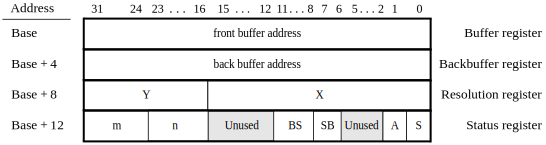
\includegraphics{figures/fig_DMA_ctrl.pdf}
   \end{center}
   \caption{Pixel buffer controller registers.}
	\label{fig:pixel_ctrl}
\end{figure}

~\\
\noindent
In a typical application the pixel buffer controller is used as follows. While the image
contained in the pixel buffer that is pointed to by the Buffer register is being displayed, 
a new image is drawn into the pixel buffer pointed to by the Backbuffer register. When this new
image is ready to be displayed, a pixel buffer swap is performed. Then, the pixel buffer 
that is now pointed to by the Backbuffer register, which was already displayed, is cleared and 
the next new image is drawn. In this way, the next image to be displayed is always drawn into
the ``back'' pixel buffer, and the ``front'' and ``back'' buffer pointers are swapped when 
the new image is ready to be displayed. Each time a swap is performed software has to 
synchronize with the VGA controller by waiting until the $S$ bit in the Status register becomes 0.

\noindent
\section*{Part I}

\noindent
You are to create a character device driver that controls the VGA display.
Your driver should use the file {\it /dev/video} to communicate with the user. Reading
from this file should return the character string ``\texttt{ccc rrr}'', where the three-digit
decimal number \texttt{ccc} is the number of columns in the VGA screen, and \texttt{rrr} is
the number of rows. One way to read from the device driver is to type a command such as
\texttt{cat /dev/video} on a Linux Terminal window. The device driver should support the
following commands that can be written to the file {\it /dev/video}: \texttt{clear}, 
and \texttt{pixel x,y color}. The \texttt{clear} command should erase the 
VGA screen by setting all pixels in the pixel 
buffer to the color 0 ({\it black}). The \texttt{pixel} command should set the pixel on the VGA
screen at the coordinates $(x, y)$ to the value \texttt{color}. One way to write to your
video driver is to type a command such as \texttt{echo clear $>$ /dev/video} on a Linux 
Terminal window. The command \texttt{echo "pixel 319,239 0x07E0" > /dev/video} would set the 
pixel at the bottom-right corner of the screen to the color green. 

~\\
\noindent
An outline of the required code for the character device driver is given in 
Figure~\ref{fig:video}. Lines \ref{line:includes} to~\ref{line:includes2} include header files
that are needed for the driver. Global variables that are used to access the pixel
buffer, which will be described later, are declared in lines~\ref{line:dec1} to~\ref{line:dec2}.
Line~\ref{line:vars} is a placeholder for the declarations of function prototypes and variables
that are needed for the character device driver. Prototypes have to be declared for the functions
that are executed when opening, reading, writing, and closing the driver. A variables of type 
\texttt{miscdevice} has to be declared and initialized in
the function {\it start\_video}, shown in lines~\ref{line:start1} to~\ref{line:start2},
which is executed when the video driver is inserted into the Linux kernel. Refer to Exercise 3 
for a more detailed discussion about the functions and variables that are needed for character
device drivers.

~\\
\noindent
To provide the kernel module with access to the FPGA light-weight bridge, line~\ref{line:c1} 
calls the \texttt{ioremap\_nocache} function. Information about this function, and the
FPGA light-weight bridge, can be found in the tutorial {\it Using Linux on DE-series Boards}.
Line~\ref{line:c2} computes the base address for the pixel buffer controller registers, 
which are illustrated in Figure~\ref{fig:pixel_ctrl}. This address is then passed to the
function named \texttt{get\_screen\_specs}, which reads the {\it Resolution} register in
the pixel controller, so that it can use this information to set the global variables 
{\it resolution\_x} and {\it resolution\_y}.

~\\
\noindent
In Line~\ref{line:c3} \texttt{ioremap\_nocache} is called again, to map the physical
addresses of the pixel buffer into virtual addresses. This code assumes that the pixel
buffer is in its default location, which is within the FPGA on-chip memory. The
\texttt{clear\_screen} function is then called, which is used to set all pixels in the
pixel buffer to the color 0, which is {\it black}. 

\lstset{language=C,numbers=left,escapechar=|}
\begin{figure}[h]
\begin{center}
\begin{minipage}[t]{15 cm}
\begin{lstlisting}[name=dots]
|\label{line:includes}|#include <linux/fs.h>               // struct file, struct file_operations
#include <linux/module.h>           // for module init and exit macros
#include <linux/miscdevice.h>       // for struct miscdev
#include <linux/uaccess.h>          // for copy_to_user, see code
#include <asm/io.h>                 // for mmap
|\label{line:includes2}|#include "address_map_arm.h"

// Declare global variables needed to use the pixel buffer
|\label{line:dec1}|void *LW_virtual;				// used to access FPGA light-weight bridge
volatile int * pixel_ctrl_ptr;	// virtual address of pixel buffer controller
int pixel_buffer;				// used for virtual address of pixel buffer
|\label{line:dec2}|int resolution_x, resolution_y;	// VGA screen size

// Declare variables and prototypes needed for a character device driver
|\label{line:vars}$\ldots$| code not shown

/* Code to initialize the video driver */
|\label{line:start1}|static int _|$\,$|_init start_video(void) {
    // initialize the miscdevice data structures
    |$\ldots$| code not shown

    // generate a virtual address for the FPGA lightweight bridge
    |\label{line:c1}|LW_virtual = ioremap_nocache (0xFF200000, 0x00005000);
    if (LW_virtual == 0)
        printk (KERN_ERR "Error: ioremap_nocache returned NULL\n");

    // Create virtual memory access to the pixel buffer controller
    |\label{line:c2}|pixel_ctrl_ptr = (unsigned int *) (LW_virtual + 0x00003020);
    get_screen_specs (pixel_ctrl_ptr); // determine X, Y screen size

    // Create virtual memory access to the pixel buffer
    |\label{line:c3}|pixel_buffer = (int) ioremap_nocache (0xC8000000, 0x0003FFFF); 
    if (pixel_buffer == 0)
        printk (KERN_ERR "Error: ioremap_nocache returned NULL\n");

    /* Erase the pixel buffer */
    clear_screen ( );
    return 0;
|\label{line:start2}|}
\end{lstlisting}
\end{minipage}
\caption{An outline of the video-driver code (Part $a$).}
\label{fig:video}
\end{center}
\end{figure}
\clearpage
\newpage
\lstset{language=C,numbers=left,escapechar=|}
\begin{center}
\begin{minipage}[t]{12.5 cm}
\begin{lstlisting}[name=dots]
void get_screen_specs(volatile int * pixel_ctrl_ptr) {
    |$\ldots$| code not shown
}
void clear_screen( ) {
    |$\ldots$| code not shown
}
void plot_pixel(int x, int y, short int color) {
    |$\ldots$| code not shown
}
static void _|$\,$|_exit stop_video(void) {
    /* unmap the physical-to-virtual mappings */
    iounmap (LW_virtual);
    iounmap ((void *) pixel_buffer);

    /* Remove the device from the kernel */
    |$\ldots$| code not shown
}
static int device_open(struct inode *inode, struct file *file) {
    return SUCCESS;
}
static int device_release(struct inode *inode, struct file *file) {
    return 0;
}
static ssize_t device_read(struct file *filp, char *buffer, size_t length, loff_t *offset) {
    |$\ldots$| code not shown
}

static ssize_t device_write(struct file *filp, const char *buffer, size_t length, loff_t *offset) {
    |$\ldots$| code not shown
}

MODULE_LICENSE("GPL");
module_init (start_video);
module_exit (stop_video);
\end{lstlisting}
~\\
Figure \ref{fig:video}. An outline of the video-driver code (Part $b$).
\end{minipage}
\end{center}

~\\
\noindent
Part $b$ of Figure~\ref{fig:video} gives an outline for the rest of the functions that are
required for the character device driver. A detailed discussion of these functions can be
found in Laboratory Exercise 3.

~\\
\noindent
Perform the following:

\begin{enumerate}
\item Create a file named {\it video.c} and fill in the missing code from Figure~\ref{fig:video}.
Create a Makefile for your character device driver. Compile the code to create the 
kernel module {\it video.ko}, and insert this module into the Linux kernel. 
\item Connect a VGA monitor to the DE-series board. If you do not have access to a
monitor, then you can use the {\it VGA Emulator} that is provided in the design files for this 
exercise.  Instructions for using the VGA Emulator are given in Appendix A.
\item Test your video character device driver by using a Terminal window. Reading from the file
{\it /dev/video} should return the string ``320 240'', which provides the VGA screen size.
Use \texttt{pixel} commands to color some pixels on the screen, and send the 
\texttt{clear} command to the video driver to erase the VGA display.
\item
Create a user-level program called {\it part1.c} that reads and writes to your video device
driver. A skeleton of an example program is given in Figure~\ref{fig:part1}. Fill in the rest 
of the code so that it performs some operations using the device driver. For example, you could 
write a loop that uses \texttt{pixel} commands to fill the entire VGA screen with a certain color.
Compile your program using a command such as \texttt{gcc -Wall -o part1 part1.c}.
Test your program by trying various operations. 
\end{enumerate}

\lstset{language=C,numbers=none}
\begin{figure}[H]
\begin{center}
\begin{minipage}[t]{15 cm}
\begin{lstlisting}[name=part1]
#include <stdio.h>
#include <string.h>
#include <errno.h>
#include <fcntl.h>
#include <unistd.h>

#define video_BYTES 8			// number of characters to read from /dev/video

int screen_x, screen_y;

int main(int argc, char *argv[])
{
    int video_FD;				// file descriptor
    char buffer[video_BYTES];	// buffer for data read from /dev/video
    char command[64];			// buffer for commands written to /dev/video
    int x, y;
    
    // Open the character device driver
    if ((video_FD = open("/dev/video", O_RDWR)) == -1) {
        printf("Error opening /dev/video: %s\n", strerror(errno));
        return -1;
    }
    // Set screen_x and screen_y by reading from the driver
    |$\ldots$| code not shown
    // Use pixel commands to color some pixels on the screen
    |$\ldots$| code not shown

    close (video_FD);
    return 0;
}
\end{lstlisting}
\end{minipage}
\vspace{-0.5cm}
\caption{A program that communicates with /{\it dev}/{\it video}.}
\label{fig:part1}
\end{center}
\end{figure}

\vspace{-1cm}
\section*{Part II}

\noindent
In this part you will add a simple line-drawing algorithm to your video driver.
Drawing a line on a screen requires coloring pixels between two coordinates $(x_1,y_1)$ and 
$(x_2,y_2)$, such that the pixels represent the desired line as closely as possible. Consider 
the example in Figure~\ref{fig:line_drawing}, where we want to draw a line between 
coordinates $(1,1)$ and $(12,5)$. The squares in the figure represent the location and 
size of pixels on the screen. As indicated in the figure, we cannot draw the line 
precisely---we can only draw a shape that is similar to the line by coloring the pixels that 
fall closest to the line's ideal location on the screen.

\begin{figure}[h!]
   \begin{center}
			  \includegraphics[scale=0.8]{figures/fig_line_drawing}
   \end{center}
   \caption{Drawing a line between coordinates $(1,1)$ and $(12,5)$.}
	\label{fig:line_drawing}
\end{figure}

~\\
\noindent
We can use algebra to determine which pixels to color. This is done by using the end points and 
the slope of the line. The slope of our example line is $slope = (y_2 - y_1)/(x_2 - x_1) = 4/11$. 
Starting at point $(1,1)$ we move along the $x$ axis and compute the $y$ coordinate for the 
line as follows:
\begin{eqnarray*}
y = y_1 + slope \times (x - x_1)
\end{eqnarray*}
\noindent
Thus, for column $x = 2$, the $y$ location of the pixel is
$1 + \frac{4}{11} \times (2-1) = 1 \frac{4}{11}$. 
Since pixel locations are defined by integer values we round the $y$ coordinate to the nearest 
integer, and determine that in column $x = 2$ we should color the pixel at $y = 1$. For
column $x = 3$ we perform the calculation $y = 1 + \frac{4}{11} \times (3-1) = 1
\frac{8}{11}$, and round the result to $y = 2$.  Similarly, we perform such computations 
for each column between $x_1$ and $x_2$.

~\\
\noindent
The approach of moving along the $x$ axis has drawbacks when a line is steep. A steep line
spans more rows than it does columns, and hence has a slope with absolute value greater than~1.
In this case our calculations will not produce a smooth-looking line.  Also, if the line
is vertical we cannot use the slope to make a calculation.  To address this 
problem, we can alter the algorithm to move along the $y$ axis when a line is steep. With 
this change, we can implement a line-drawing algorithm known as {\it Bresenham's algorithm}.
A key property of this algorithm is that all variables are {\it integers}.
Pseudo-code for this algorithm is given in Figure~\ref{fig:bresenham}. The first 15
lines of the algorithm make the needed adjustments depending on whether or not the line is
steep. Then, in lines 17 to 22 the algorithm increments the {\it x} variable 1 step at a time
and computes the {\it y} value. The {\it y} value is incremented when needed to stay as
close to the ideal location of the line as possible. Bresenham's algorithm calculates an
{\it error} variable to decide whether or not to increment each {\it y} value. 
The {\it error} variable takes into account the relative difference
between the width of the line ({\it deltax}) and height of the line ({\it deltay}) in deciding
how often {\it y} should be incremented.  The version
of the algorithm shown in Figure~\ref{fig:bresenham} uses only integers to perform
all calculations.

\begin{figure}[h]
\begin{center}
\begin{minipage}[t]{12.5 cm}
\begin{lstlisting}[numbers=left,name=bresenham]
draw_line(x0, x1, y0, y1)
	is_steep = (abs(y1 - y0) > abs(x1 - x0))
	if is_steep then
		swap(x0, y0)
		swap(x1, y1)
	if x0 > x1 then
		swap(x0, x1)
		swap(y0, y1)

	deltax = x1 - x0
	deltay = abs(y1 - y0)
	error = -(deltax / 2)
	y = y0
	|\label{line:adjust}|if y0 < y1 then y_step = 1 else y_step = -1

	|\label{line:f1}|for x from x0 to x1
		if is_steep then draw_pixel(y,x) else draw_pixel(x,y)
		error = error + deltay
		if error |$\ge$| 0 then
			y = y + y_step
			|\label{line:f2}|error = error - deltax
\end{lstlisting}
\end{minipage}
\caption{Pseudo-code for a line-drawing algorithm.}
\label{fig:bresenham}
\end{center}
\end{figure}

\newpage
\noindent
Perform the following:

\begin{enumerate}

\item Using your character device driver from Part I it would be possible to draw lines by 
repeatedly sending \texttt{pixel} commands to the driver. However, this would be an inefficient
approach due to the large number of writes that may have to be made to the file {\it /dev/video}.
A better approach is to implement a line-drawing algorithm within the video driver. Augment
your driver by adding a function called {\it draw\_line} that implements Bresenham's algorithm.
Also, add a new command \texttt{line x1,y1 x2,y2 color} that invokes this function.
		  
\item Remove your kernel module from Part I, recompile the new version which includes the
\texttt{line} command, and then re-insert the module back into the kernel.
\item Use the \texttt{echo} command in a Terminal window to test your line-drawing function.
\item Part of a user-level program that draws a few lines on the VGA screen is depicted in
Figure~\ref{fig:part2}. Fill in the missing parts of this program. Compile and test it.
\end{enumerate}

\lstset{language=C,numbers=none}
\begin{figure}[H]
\begin{center}
\begin{minipage}[t]{15 cm}
\begin{lstlisting}[name=part2]
#include <stdio.h>
|$\ldots$| other include statements not shown

#define video_BYTES 8	// number of characters to read from /dev/video

int screen_x, screen_y;

int main(int argc, char *argv[])
{
    int video_FD;                       // file descriptor
    char c, video_buffer[video_BYTES];  // buffer for video char data
    char command[64];                   // buffer for command data
    
    // Open the character device driver
    if ((video_FD = open("/dev/video", O_RDWR)) == -1) {
        printf("Error opening /dev/video: %s\n", strerror(errno));
        return -1;
    }
	
    // Read VGA screen size from the video driver
    |$\ldots$| code not shown

    /* Draw a few lines */
    sprintf (command, "line %d,%d %d,%d %X\n", 0, screen_y - 1, screen_x - 1, 0, 0xFFE0);	// yellow
    write (video_FD, command, strlen(command));
    sprintf (command, "line %d,%d %d,%d %X\n", 0, screen_y - 1, 
        (screen_x >> 1) - 1, 0, 0x07FF);	// cyan
    write (video_FD, command, strlen(command));
        (screen_x >> 2) - 1, 0, 0x07E0);	// green
    write (video_FD, command, strlen(command));
    |$\ldots$| etc.

    close (video_FD);
    return 0;
}
\end{lstlisting}
\end{minipage}
\caption{A user-level program that draws a few lines.}
\label{fig:part2}
\end{center}
\end{figure}

\pagebreak

\noindent
\section*{Part III}

\noindent
Animation is an exciting part of computer graphics. Moving a displayed object is an illusion 
created by showing this same object at different locations on the screen. A simple way to
``move'' an object is to first draw the object at one position, and then after a short time erase 
the object and draw it again at another nearby position.

~\\
\noindent
To realize animation it is necessary to move objects at regular time intervals. The VGA controller 
in the DE1-SoC Computer redraws the screen every $1/60^{th}$ of a second. Since the image on 
the screen cannot change more often than that, it is reasonable to control an animation
using this unit of time.

~\\
\noindent
To ensure that you change the image only once every $1/60^{th}$ of a second, use the 
pixel buffer controller to synchronize with the vertical synchronization cycle of the VGA 
controller. As we discussed in the background section of this exercise, synchronizing with the 
VGA controller can be accomplished by writing the value~1 into the {\it Buffer} register in the 
pixel buffer controller, and then waiting until bit $S$ of the {\it Status} register becomes 
equal to 0. For this part of the exercise you do not need to use a back buffer, so ensure
that the {\it Buffer} and {\it Backbuffer} addresses in the pixel buffer controller are the 
same. In this approach, a pixel buffer ``swap'' can be used as a way of synchronizing with 
the VGA controller via the {\it S} bit in the {\it Status} register.

~\\
\noindent
Perform the following:

\begin{enumerate}

\item Augment your video driver so that it includes the ability to perform a pixel buffer swap,
as described above. Also add a new command to the video driver, called \texttt{sync}, that allows
a user-level program to synchronize with the VGA controller. Remove the previous version
of the driver from the Linux kernel, and compile and insert the new version.
\item Write a user-level program that creates a simple animation using your video driver. The
animation should ``move'' a horizontal line up and down on the screen and ``bounce'' the line 
off the top and bottom edges of the display. Your program should first clear the screen and
draw the line at a starting row on the screen. Then, in an endless loop you should perform
a VGA synchronization, erase the line (by drawing the line using black), and redraw it one row
above or below the last one. When the line reaches the top, or bottom, of the screen it should
start moving in the opposite direction.

\item Compile and execute your code. Notice how long it takes for the 
horizontal line to move through the 240 lines of the VGA display. It should take 
$240 \times 1/60 = 4$ seconds.
\end{enumerate}

\noindent
\section*{Part IV}

\noindent
Having gained the basic knowledge, you can now create a more interesting animation.
You are to create an animation of eight small filled rectangles on the screen. These rectangles 
should appear to be moving continuously and ``bouncing'' off the edges of the screen. The 
rectangles should be connected with lines to form a chain. An illustration of the animation 
is given in Figure~\ref{fig:animation_example}. Part $a$ of the figure shows one position
of the rectangles with arrows that indicate the directions of movement, and 
Figure~\ref{fig:animation_example}$b$ shows a subsequent position of the rectangles. 
In each step of your animation each of the rectangles should appear to ``move'' on a diagonal 
line: up/left, up/right, down/left, or down/right. Move the rectangles one
row and one column at a time on the VGA screen.

\begin{figure}[h!]
   \begin{center}
       \includegraphics[scale = 0.5]{figures/fig_animation_example.pdf}
   \end{center}
	\vspace{-0.5cm}
   \caption{Two instants of the animation.}
	\label{fig:animation_example}
\end{figure}

~\\
\noindent
To make the animation look slightly different each time you run it, you can use the C library
function {\it rand ()} to help calculate initial positions for each of the rectangles, and to
determine their directions of movement. 

~\\
\noindent
Perform the following:

\begin{enumerate}
\item Augment your video driver to add a new command: \texttt{box x1,y1 x2,y2 color}. Remove
the previous version of the driver from the Linux kernel, and compile and insert the new version.
\item Write a user-level program to implement your animation. Use both a front and back buffer 
in your program, so that you can avoid making changes to the image while it is being displayed 
by the pixel buffer controller. If you are using the DE1-SoC Computer, then in addition to 
placing one pixel buffer in the FPGA on-chip memory, you can place the other buffer in 
the SDRAM memory, which has the starting address \texttt{0xC0000000}. This choice is also
available in the DE10-Standard Computer. If using the DE10-Nano Computer, then place both pixel
buffers in the FPGA on-chip memory; if the first buffer starts at address \texttt{0xC8000000}, 
then the other buffer can begin at \texttt{0xC8000000} $+$ $(512 \times 256)$.
An outline of a suitable program is illustrated in 
Figure~\ref{fig:part4}. Compile, execute, and test your program.

\item Experiment with your code by modifying it to use just a single pixel buffer (simply
change the address of the back buffer to be the same as the front buffer). Notice how the
animation differs with this change.
\end{enumerate}

\section*{Part V}

\noindent
For this part of the exercise you are to enhance the animation from Part~IV so that during the
animation the following changes can take place:

\begin{enumerate}
\item
The speed of movement of the rectangles can be increased or decreased
\item
The number of rectangles can be increased or decreased
\item
The lines between rectangles can be drawn or not drawn
\end{enumerate}
\noindent
In Part IV the animation speed was set by the 1/60 seconds VGA vertical synchronization time.
One way to control the speed of animation is to make use of a timer. You can use the
{\it nanosleep} timer that is provided by the Linux kernel. In this scheme, the main 
program would draw the next step of the animation each time the timer expires.  Lengthening 
the timeout would produce a slower animation, and shortening the timeout would speed up the 
animation. The maximum speed of the animation would be limited by the 1/60 seconds VGA
synchronization time, as it was in Part IV. To cause the animation to appear to move more 
quickly than in Part IV, you have to increase the screen-distance that the rectangles move
in each step of the animation.

~\\
\noindent
Perform the following:

\begin{enumerate}
\item Implement the animation control discussed above. All of your code changes
should be done in a user-level program; you do not need to modify your video driver.
The user should be able to control the animation by using the KEY pushbuttons and SW slide
switches. If you are using the DE1-SoC or DE10-Standard boards, then implement the actions 
shown in Table~\ref{tab:action1}. For the DE10-Nano board, use the actions given in 
Table~\ref{tab:action2}, because this board has fewer switches. 
When any of the SW switches is set to the ``on'' position the lines between objects should 
not be drawn; only when all SW switches are set to the ``off'' position should the 
lines appear. Access both the SW and KEY switches by using their respective character 
device drivers. 

\item Compile and test your animation code.
\newpage
\lstset{language=C,numbers=none}
\begin{figure}[H]
\begin{center}
\begin{minipage}[t]{15 cm}
\begin{lstlisting}[name=part4]
#include <stdio.h>
|$\ldots$| other include statements not shown

/* Declare global variables needed for the animation */
|$\ldots$| code not shown

void draw (int);

volatile sig_atomic_t stop;
void catchSIGINT(int signum) {
    stop = 1;
}

int main(int argc, char *argv[])
{
    int i, video_FD;    // file descriptor
    |$\ldots$| other declarations not shown
    
    // catch SIGINT from ^C, instead of having it abruptly close this program
    signal(SIGINT, catchSIGINT);
    
    |$\ldots$| code to open the video driver shown

    // set random initial position and "delta" for all rectangle boxes
    |$\ldots$| code not shown

    while (!stop) {
        draw (video_FD);
        // sync with VGA display 
        write (video_FD, "sync", 5);
    }
    close (video_FD);
    return 0;
}

/* Code that draws the animation objects, and updates their positions */
void draw(int fd) {
    |$\ldots$| code not shown
}
\end{lstlisting}
\end{minipage}
\caption{A user-level program that makes an animation.}
\label{fig:part4}
\end{center}
\end{figure}
\end{enumerate}

\begin{table}[h]
\caption{Animation control for the DE1-SoC and DE10-Standard boards.}
~\\
\centering
\label{tab:action1}
\begin{tabular}{c|p{10cm}}
{\bf KEY} & {\bf Action} \\ \hline
\rule{0cm}{12pt}{\it KEY}$_0$ & The speed of animation should be increased by some noticeable amount \\
{\it KEY}$_1$ & The speed of animation should be decreased by some noticeable amount \\
{\it KEY}$_2$ & The number of displayed objects should be increased by one \\
{\it KEY}$_3$ & The number of displayed objects should be decreased by one \\
\end{tabular}
\end{table}

\begin{table}[h]
\caption{Animation control for the DE10-Nano board.}
~\\
\centering
\label{tab:action2}
\begin{tabular}{c|p{13cm}}
{\bf KEY} & {\bf Action} \\ \hline
\rule{0cm}{12pt}{\it KEY}$_0$ & Each press of this key should increase the speed of animation by a noticeable amount, until some maximum is reached. After hitting the maximum speed, further presses of this KEY should reduce the animation speed, until some minimum is reached.\\
{\it KEY}$_1$ & Pressing this key should increase the number of displayed objects by some quantity, up to a maximum. After reaching the maximum, further presses of this KEY should reduce the number of displayed objects.\\
\end{tabular}
\end{table}

\section*{Part VI}

\noindent
We mentioned in the background section of this exercise that the image displayed by the VGA
controller can be derived from both a {\it pixel} buffer, and a {\it character} buffer. For 
this part of the exercise you are to enhance your video driver so that it supports the
display of text characters.  The character buffer is stored in FPGA on-chip memory in the 
DE1-SoC Computer. Figure \ref{fig:chars}$a$ depicts the character buffer for the VGA
display, which has a resolution of 80 $\times$ 60 characters. Each character occupies an
8 $\times$ 8 block of pixels on the screen. Characters are stored in each of the locations
shown in Figure \ref{fig:chars}$a$ using their ASCII codes; when you store an ASCII character into
the buffer, a corresponding pattern of pixels is automatically generated and displayed using 
a built-in font. Part~$b$ of Figure~\ref{fig:chars} shows
that characters are addressed in the memory by using the combination of a {\it base} address,
which has the value (C9000000)$_{16}$, and an {\it x,y} offset. Using this scheme, the
character at coordinates $(0,0)$ has the address (C9000000)$_{16}$, 
$(1,0)$ has the address {\it base} $+$ (000000 0000001)$_2$ = (C9000001)$_{16}$, 
$(0,1)$ has the address {\it base} $+$ (000001 0000000)$_2$ = (C9000080)$_{16}$, and 
the character at location $(79,59)$ has the address {\it base} $+$ (111011 1001111)$_2$ = 
(C9001DCF)$_{16}$. 

\begin{figure}[h]
   \begin{center}
       \includegraphics{figures/fig_chars.pdf}
   \end{center}
   \caption{Character buffer coordinates and addresses.}
	\label{fig:chars}
\end{figure}

~\\
\noindent
The character buffer has an associated controller, with a
register interface like the one shown in Figure~\ref{fig:pixel_ctrl}. The base address of
this controller is {\sf 0xFF203030}.  You can read from the
{\it Resolution} register to obtain the number of text columns ($X$) and rows ($Y$) on
the screen. For the VGA screen, the values will be 80 columns $\times$ 60 rows.

~\\
\noindent
Perform the following:

\begin{enumerate}
\item Enhance your kernel module from Part V by adding two new commands: \texttt{erase}, and 
\texttt{text x,y string}. The \texttt{erase} command should clear all characters from the VGA 
screen (by filling the screen with the ` ' space character).
The \texttt{text} command should store the ASCII characters in the {\it string} into coordinates
starting at \texttt{(x, y)} in the character buffer. Remove the previous version of your 
video driver from the Linux kernel, and compile and insert the new version.
\item Augment your user-level program from Part V so that it displays, in the upper-left corner 
of the screen, the number of video frames that have been drawn. Using the default animation speed,
the frame counter should increment at the rate of 60 times per second.
\item Compile and test your animation.
\end{enumerate}

\newpage
\section*{Appendix A~~~~ Using the VGA Emulator}

The design files for this exercise include a folder named \texttt{VGA\_emulator}. Copy
this folder in its entirety onto the SD Card of your DE1-SoC board. The VGA emulator is a
program that monitors the contents of the VGA pixel and character buffers, and displays a
corresponding image in a window within the VNC Viewer. To use this program, open the VNC
Viewer, and then open a Terminal window within the VNC Viewer. As shown in
Figure~\ref{fig:emulator}, in
the \texttt{VGA\_emulator} directory execute the {\it vga} program. Any video output that
is present in the pixel or character buffers will be shown in the emulator window. In this
example, we have executed a command in a Terminal window (via {\it putty}) to insert a 
{\it video.ko} driver. Then, we sent commands to this driver to draw some lines and text in 
the VGA output. If a VGA monitor were connected to the DE1-SoC board, then the same image 
shown in the emulator window would be displayed there. 

\begin{figure}[h]
   \begin{center}
       \includegraphics{figures/fig_emulator.png}
   \end{center}
   \caption{VGA Emulator.}
	\label{fig:emulator}
\end{figure}

\vskip 0.8in
\noindent
\newpage
\input{\CommonDocsPath/copyright.tex}

\end{document}
